\begin{tikzpicture}[font=\scriptsize, >={Stealth[length=2mm]}, scale=1.15]
  % dock cage (top view), entry faces left
  \fill[fill={white!70!blue}] (8.0,-0.75) rectangle (9.6,0.75);
  \fill[white] (8.0,-0.55) rectangle (9.4,0.55);
  \draw[thick] (8.0,-0.75) rectangle (9.6,0.75);
  \draw[thick] (8.0,-0.55) rectangle (9.4,0.55);
  \node at (8.8,1.05) {dock (top view)};
  % entry axis
  \draw[dashed] (0.2,0) -- (8.0,0);
  \node at (5.2,0.25) {\tiny entry axis};
  % blackout zone
  \fill[red!12] (7.6,-0.6) rectangle (8.0,0.6);
  \node[red!60!black, align=center] at (6.3,-1.45) {\tiny vision blackout $<$ 0.05 m};
  \draw[red!60!black, ->] (6.7,-1.3) -- (7.8,-0.5);
  % entry plane + aperture
  \draw[<->] (8.1,-0.55) -- (8.1,0.55);
  \node[align=center] at (9.3,-1.15) {\tiny aperture\\ \tiny $\pm$0.15 m};
  \draw[->] (9.0,-0.98) -- (8.15,-0.4);
  % seat point
  \draw[thick] (7.2,-0.15) -- (7.2,0.15);
  \node[align=center] at (6.1,0.95) {\tiny seat: 0.10 m,\\ \tiny $\pm$0.03 m lateral};
  \draw[->] (6.4,0.72) -- (7.15,0.2);
  % standoff
  \node at (3.4,0) {$\times$};
  \node[align=center] at (3.4,0.55) {\tiny standoff point\\ \tiny (coarse target)};
  % vehicle (side-view render, front faces the dock)
  \node[inner sep=0] (rov) at (1.4,0) {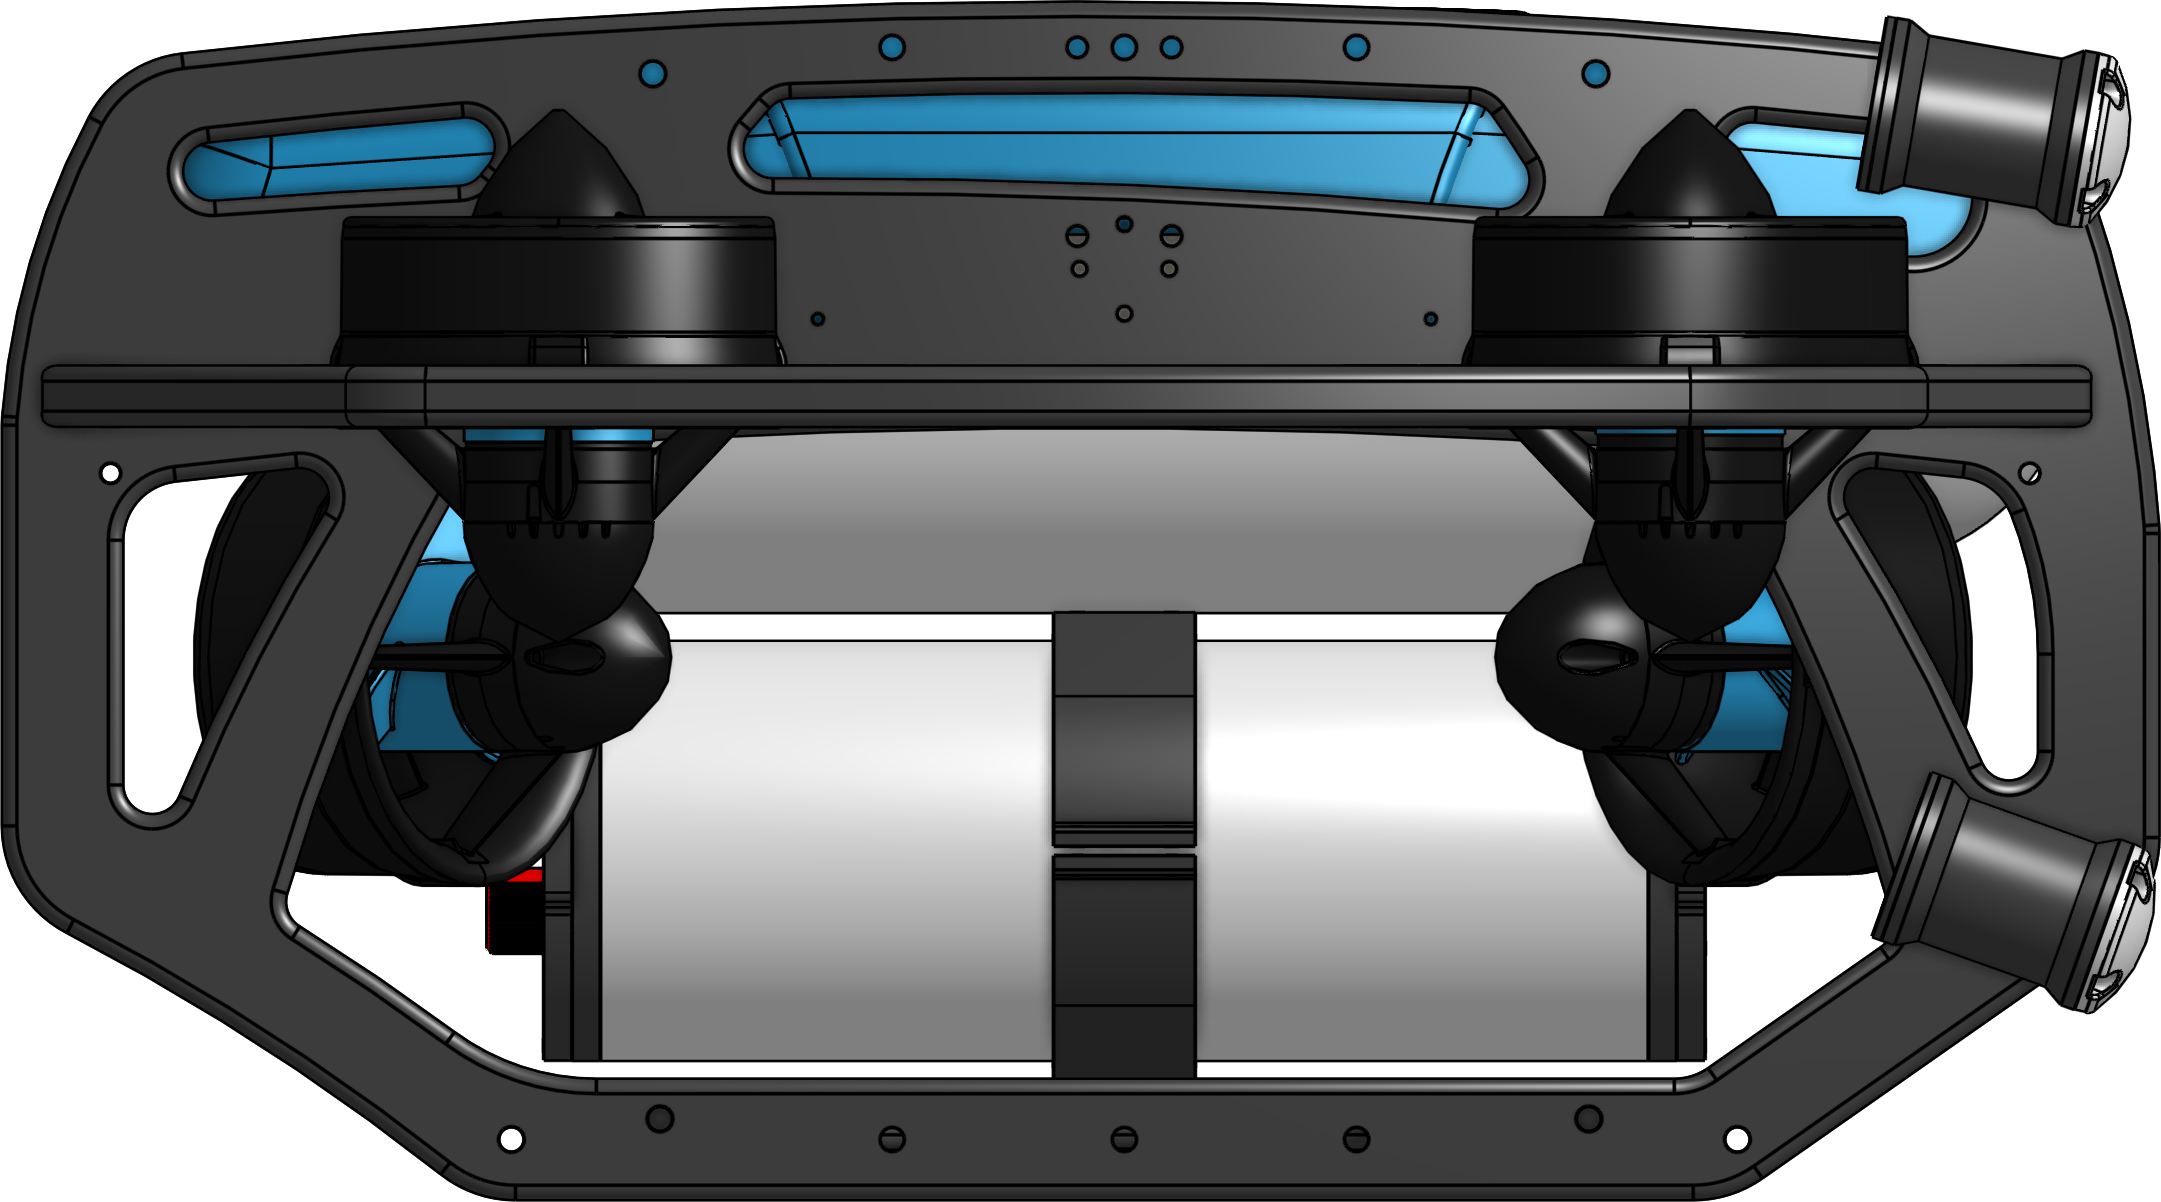
\includegraphics[width=18mm]{Images/BROV2_heavy_side.png}};
  \node at (1.4,-0.75) {\tiny ROV};
  \draw[->] (rov.east) ++(1mm,0) -- (3.15,0);
  % distance annotations
  \draw[|<->|] (3.4,-0.9) -- (8.0,-0.9);
  \node at (5.0,-1.1) {\tiny 1.0 m (not to scale)};
\end{tikzpicture}
